% @(#) This-module-01-Overview-Growth-2014-DQ.tex:
% Last edited: Mon Jun 30 15:14:40 2014 - Danny Quah (dquah@LSE016404)
% $
% Revision History:
%  % Mon Jun 30 15:13:23 2014 - Danny Quah (dquah@LSE016404)
%    First draft, cloned from db-Templates
% $
% $Log$
%%
%% Prologue in 00-Lecture-Driver/This-module-00-Lectures-2014-DQ.tex;
%% run this file from there
%% %%%%%%%%%%%%
\title[Overview: Growth]{EC4880: 1.~Overview---Growth and Evolution}
%
%---------------------------------------------------------------------%
% LOCAL DEFINES %
%---------------------------------------------------------------------%
% %%% DOCUMENT %%%
\begin{document}
 \frame{\titlepage}
%%%%%%%%%%%%%%%%%%%%%%%%%%%%%%%%%%%%%%%%%%%%%%%%%%
\begin{frame}
 \frametitle{OUTLINE}
 \tableofcontents
\end{frame}
%%%%%%%%%%%%%%%%%%%%%%%%%%%%%%%%%%%%%%%%%%%%%%%%%%
\section{The Global Economic Landscape}

%---------------------------------------------------------------------%
% FRAME %
%---------------------------------------------------------------------%
%% US / exponential growth ++
\begin{frame}[plain]
 % \frametitle{}
 \begin{center}
 \includegraphics[width=0.8\textwidth]%
  {\DirCode/{2014.03-World-Growth/figure/US-trend1}}
 \end{center}
\end{frame}
%---------------------------------------------------------------------%
% FRAME %
%---------------------------------------------------------------------%
%% UK / exponential growth
\begin{frame}[plain]
 % \frametitle{}
 \begin{center}
 \includegraphics[width=0.8\textwidth]%
  {\DirCode/{2014.03-World-Growth/figure/UK-trend1}}
 \end{center}
\end{frame}
%---------------------------------------------------------------------%
% FRAME %
%---------------------------------------------------------------------%
%% China / exponential growth
\begin{frame}[plain]
 % \frametitle{}
 \begin{center}
 \includegraphics[width=0.8\textwidth]%
  {\DirCode/{2014.03-World-Growth/figure/CN-trend1}}
 \end{center}
\end{frame}
%% Lights
%% BRICs / Goldman Sachs

%---------------------------------------------------------------------%
% FRAME %
%---------------------------------------------------------------------%
%% In perspective
\begin{frame}[plain]
 % \frametitle{}
 \begin{center}
 \includegraphics[width=0.8\textwidth]%
  {\DirCode/{2014.03-World-Growth/figure/US-UK-China}}
 \end{center}
\end{frame}

%---------------------------------------------------------------------%
% FRAME %
%---------------------------------------------------------------------%
\begin{frame} \frametitle{Empirical Lessons}
\begin{enumerate}
 \item{Fitted trends tend artificially to induce cyclicality. But the
 out-of-sample extrapolation does give useful information.}
 \item{US, UK trend fit vs China's out-of-sample growth}
 \item{Cross comparison informs on relative cross-section performance,
 not just in contrast to own history.}
\end{enumerate}
 \end{frame}
%---------------------------------------------------------------------%

%%%%%%%%%%%%%%%%%%%%%%%%%%%%%%%%%%%%%%%%%%%%%%%%%%
\section{How Do Economists Think About This?}
%---------------------------------------------------------------------%
% FRAME %
%---------------------------------------------------------------------%
\begin{frame}\frametitle{Growth Accounting}

\begin{align*}
 Y &= F(K, NA) \\
 K &\text{ physical capital}\\
 N &\text{ labour}\\
 A &\text{ technology (labour-augmenting)}\\
\intertext{Write}
 k &= K/N~\text{per capita stock of physical capital}\\
 \tilde{k}&=K/(NA)~\text{technology-adjusted $k$}
\end{align*}
\end{frame}
%---------------------------------------------------------------------%
% FRAME %
%---------------------------------------------------------------------%
\begin{frame}\frametitle{Growth Dynamics}

Then (under ``constant returns to scale'')
\begin{equation*}
 y = Y/N = F(K/NA, 1) \times A = f(\widetilde{k}) \times A . 
\end{equation*}

Per capita GDP grows from the accumulation of $k$ (physical capital)
and progress in $A$ (technology).

\begin{equation*}
 \log y = \log f(\widetilde{k}) + \log A . 
\end{equation*}

\begin{enumerate}
 \item{Economic growth comes from investment to build machines and
 from investment to accumulate knowledge and advance technology.}
 \item{Limits to growth from just accumulating capital:  Declining
 marginal returns in production function}
 \item{R\&D and other knowledge-based activity drive $A$.}
 \item{``Human capital'':  Is it like physical capital or is it a
 driver for technology?}
\end{enumerate}

\end{frame}

%% f(k) picture - no need

%---------------------------------------------------------------------%
% FRAME %
%---------------------------------------------------------------------%
%% Growth and convergence
\begin{frame}\frametitle{Growth and Convergence}
\begin{center}
\begin{columns}
 \begin{column}{0.45\textwidth}
 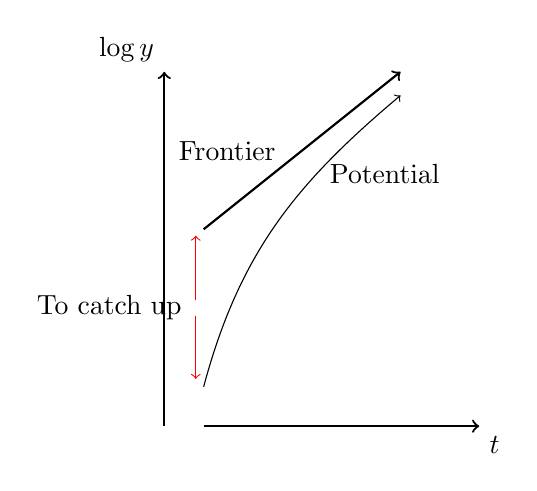
\begin{tikzpicture}
 \draw[thick,->] (0.5, 0) -- (4.0, 0) node[anchor=north west] {$t$} ;
 \draw[thick,->] (0, 0) -- (0, 4.5) node[anchor=south east] {$\log y$} ;

 \draw[thick,->] (0.5, 2.5) -- (3.0, 4.5) ;

 \draw[->] plot [smooth] (0.5, 0.5) to[out=75,in=-140] (3.0, 4.2) ;

 \node at (0.8, 3.5) {Frontier} ;
 \node at (2.8, 3.2) {Potential} ;

 \node at (-0.7, 1.5) {To catch up} ;
 \draw[red,->] (0.4, 1.6) -- (0.4, 2.42) ;
 \draw[red,->] (0.4, 1.4) -- (0.4, 0.60) ;

 \end{tikzpicture}
 \end{column}
 \begin{column}{0.5\textwidth}
  1.~Frontier describes $\log A$ increasing from technological progess.
  2.~Catch-up represents accumulation in physical capital.
  3.~Fast growth occurs when an economy is poorer.
 \end{column}
\end{columns}
\end{center}
\end{frame}

%%%%%%%%%%%%%%%%%%%%%%%%%%%%%%%%%%%%%%%%%%%%%%%%%%
\section{BRICs++ :  Names and Places. Not Just Subscript $j$}

%---------------------------------------------------------------------%
% FRAME %
%---------------------------------------------------------------------%
%% BRICs

%% From
{ % all template changes are local to this group.
    \setbeamertemplate{navigation symbols}{}
    \begin{frame}[plain]
        \begin{tikzpicture}[remember picture,overlay]
            \node[at=(current page.center)] {
                \includegraphics[width=\paperwidth]%
                {\DirImages/BRIC-2009}
            };
        \end{tikzpicture}
     \btVFill
        \hspace{-0.9cm}\noindent{\linespread{0.5}\selectfont
        \textcolor{black}{\tiny
        Source: Goldman Sachs 2010
        }
        \par
        }
     \end{frame}
}

%---------------------------------------------------------------------%
% FRAME %
%---------------------------------------------------------------------%
%% BRICs

%% From
{ % all template changes are local to this group.
    \setbeamertemplate{navigation symbols}{}
    \begin{frame}[plain]
        \begin{tikzpicture}[remember picture,overlay]
            \node[at=(current page.center)] {
                \includegraphics[width=\paperwidth]%
                {\DirImages/BRIC-2050}
            };
        \end{tikzpicture}
     \btVFill
        \hspace{-0.9cm}\noindent{\linespread{0.5}\selectfont
        \textcolor{black}{\tiny
        Source: Goldman Sachs 2010
        }
        \par
        }
     \end{frame}
}

%%%%%%%%%%%%%%%%%%%%%%%%%%%%%%%%%%%%%%%%%%%%%%%%%%
\section{The World's Economic Centre of Gravity}

%---------------------------------------------------------------------%
% FRAME %
%---------------------------------------------------------------------%
%% Lights

%% From
%% http://tex.stackexchange.com/questions/3915/image-on-full-slide-in-beamer-package
{ % all template changes are local to this group.
    \setbeamertemplate{navigation symbols}{}
    \begin{frame}[plain]
        \begin{tikzpicture}[remember picture,overlay]
            \node[at=(current page.center)] {
                \includegraphics[width=\paperwidth]%
                {\DirImages/{NASA/DQ-Land-Lights}}
%{\DirImages/{NASA/Final-from-Design-Unit/land-lights-16384lightened-lower}}
            };
        \end{tikzpicture}
     \btVFill
        \hspace{-0.9cm}\noindent{\linespread{0.5}\selectfont
        \textcolor{white}{\tiny
        Source: DMSP data courtesy Marc
        Imhoff of NASA GSFC and Christopher Elvidge of NOAA
        NGDC. Image by Craig Mayhew and Robert Simmon, NASA Earth
        Observatory. 
        }
        \par
        }
     \end{frame}
}

%---------------------------------------------------------------------%
% FRAME %
%---------------------------------------------------------------------%
%% WECG
{ % all template changes are local to this group.
    \setbeamertemplate{navigation symbols}{}
    \begin{frame}[plain]
        \begin{tikzpicture}[remember picture,overlay]
            \node[at=(current page.center)] {
                \includegraphics[width=\paperwidth]%
                {\DirImages/{2010.09.27-LSE-Research-DQ-Map}}
            };
        \end{tikzpicture}
     \btVFill
        \hspace{-0.9cm}\noindent{\linespread{0.5}\selectfont
        \textcolor{black}{\tiny
        Source: D. Quah (2011).  The World's Shifting Economic Centre of
    Gravity
        }
        \par
        }
     \end{frame}
}

%---------------------------------------------------------------------%
% FRAME %
%---------------------------------------------------------------------%
%% WECG
{ % all template changes are local to this group.
    \setbeamertemplate{navigation symbols}{}
    \begin{frame}[plain]
        \begin{tikzpicture}[remember picture,overlay]
            \node[at=(current page.center)] {
                \includegraphics[width=\paperwidth]%
                {\DirImages/{2011-Latitudinal-projection-DQ}}
            };
        \end{tikzpicture}
     \btVFill
        \hspace{-0.9cm}\noindent{\linespread{0.5}\selectfont
        \textcolor{black}{\tiny
        Source: D. Quah (2011).  The World's Shifting Economic Centre of
    Gravity
        }
        \par
        }
     \end{frame}
}

%---------------------------------------------------------------------%
% FRAME %
%---------------------------------------------------------------------%
\begin{frame}\frametitle{BRICs?  Or a Great Shift East?}

\begin{enumerate}
\item{Brazil, Russia, India, China:  BRICs (via Goldman Sachs/Jim
    O'Neill)}
\item{South Africa?  Korea?  Indonesia?}
\item{The picture, however, is more of a ``Great Shift East''}
\end{enumerate}

\end{frame}

%%%%%%%%%%%%%%%%%%%%%%%%%%%%%%%%%%%%%%%%%%%%%%%%%%
\section{The Global Landscape of Poverty}

%---------------------------------------------------------------------%
% FRAME %
%---------------------------------------------------------------------%
%% The WSJ indictment

%% From
{ % all template changes are local to this group.
    \setbeamertemplate{navigation symbols}{}
    \begin{frame}[plain]
        \begin{tikzpicture}[remember picture,overlay]
            \node[at=(current page.center)] {
                \includegraphics[width=\paperwidth]%
                {\DirImages/{2005-WSJ-China-Inequality}}
            };
        \end{tikzpicture}
     \btVFill
        \hspace{-0.9cm}\noindent{\linespread{0.5}\selectfont
        \textcolor{black}{\tiny
        Source: Wall Street Journal 2005
        }
        \par
        }
     \end{frame}
}

%---------------------------------------------------------------------%
% FRAME %
%---------------------------------------------------------------------%
\begin{frame}\frametitle{World Growth and Poverty}

\begin{table}
\begin{tabularx}{0.9\textwidth}{l c c c c}
\firsthline
&1981&1990&1999&2005\\
\hline
World GDP, tn PPP\$&26&35&45&56\\
GDP per capita, PPP\$&5876&6704&7505&8662\\
World's poor, mn&1904&1815&1695&1400\\
China's poor, mn&835&683&447&208\\
Remainder, mn&1069&1132&1248&1192\\
\hline
\end{tabularx}
\end{table}
\end{frame}
%---------------------------------------------------------------------%
% FRAME %
%---------------------------------------------------------------------%
%% Dollar-Kraay

%% From
{ % all template changes are local to this group.
    \setbeamertemplate{navigation symbols}{}
    \begin{frame}[plain]
        \begin{tikzpicture}[remember picture,overlay]
            \node[at=(current page.center)] {
                \includegraphics[width=0.9\paperwidth]%
                {\DirImages/{2002.09-David.Dollar+Aart.Kraay-Growth-Good-for-Poor}}
            };
        \end{tikzpicture}
     \btVFill
        \hspace{-0.9cm}\noindent{\linespread{0.5}\selectfont
        \textcolor{black}{\tiny
        Source: Dollar and Kraay 2002
        }
        \par
        }
     \end{frame}
}

%%%%%%%%%%%%%%%%%%%%%%%%%%%%%%%%%%%%%%%%%%%%%%%%%%
\section{Conclusion}

%---------------------------------------------------------------------%
% FRAME %
%---------------------------------------------------------------------%
\begin{frame}\frametitle{Concepts to remember and use}

\begin{enumerate}
 \item{Growth and trends:  Neoclassical growth and convergence}
 \item{Size matters.  Subscripts and names and places}
 \item{BRICs or a ``Great Shift East''? WECG}
 \item{Poverty and Growth}
 \item{Disjoint global economic and political landscapes?}
\end{enumerate}

\end{frame}
%---------------------------------------------------------------------%
% (END) FRAME %
%---------------------------------------------------------------------%
%
\end{document}

\begin{frame}


\end{frame}


%
% 
% Local Variables:
% mode: TeX
% end:
% eof This-module-01-Overview-Growth-2014-DQ.tex:
